%% Force PDFLaTeX for arXiv
\pdfoutput=1

\documentclass[11pt]{amsart}
\usepackage{geometry}
\geometry{letterpaper, margin=1in}
\usepackage{amsmath,amssymb,amsthm}
\usepackage{graphicx}
\usepackage{url}
\usepackage{hyperref}

\newtheorem{lemma}{Lemma}[section]
\newtheorem{proposition}[lemma]{Proposition}
\newtheorem{remark}[lemma]{Remark}

\title{Khayyam's Triangle: Historical Restoration and the Geometry Hidden in the Numbers}

\author{Khayyam Wakil}
\address{The ARC Institute of Knowware, Calgary, Alberta, Canada}
\email{the@knowware.institute}
\date{January 2026}

\subjclass[2020]{01A30, 11B65, 28A80, 11N35}
\keywords{Pascal's triangle, Khayyam's triangle, Sierpiński fractal, Lucas's theorem, modular arithmetic, history of mathematics, cascade moduli, constitutional sieve theory}

\begin{document}

\begin{abstract}
The triangular array of binomial coefficients has been called ``Pascal's Triangle'' in the West for centuries---yet Pascal arrived 584 years after the Persian mathematician Omar Khayyam first documented it. That alone might justify a rename. But there is a stronger argument hiding in plain sight: the triangle's deepest structural property is \emph{geometric}, not combinatorial, and it belongs by mathematical character to Khayyam's tradition rather than Pascal's. Reduce the triangle's entries modulo any prime $p$ and a Sierpiński-type fractal emerges---a self-similar geometric structure invisible to Pascal's probabilistic eye, but exactly the kind of hidden geometry Khayyam spent his life finding.

This paper is the first in a six-paper program on constitutional sieve theory. The mod-3 fractal structure of Khayyam's Triangle, governed by Lucas's theorem, is the direct combinatorial ancestor of the cascade moduli framework and the level-of-distribution result $\theta_W = 5/8$ proved in the companion papers \cite{ramanujan,eisenstein}. A reader wishing to understand why the prime 3 plays a privileged role in that arithmetic program will find the answer here. This paper makes the historical and mathematical case, and shows you the fractal.
\end{abstract}

\maketitle

\tableofcontents

\section{The Wrong Man's Name}

Here is a simple question nobody seems to have asked. You know the triangular array of binomial coefficients---the one where each entry is the sum of the two above it, the one that encodes combinations, gives you Pascal's Rule, and sits in every combinatorics textbook. You call it Pascal's Triangle. But what does its deepest structural property look like, and whose mathematical instincts would have found it?

Colour every entry that is \emph{not} divisible by 3 and leave the rest blank. Do this for row after row, hundreds of rows deep. What emerges is not a triangle. It is a fractal---an infinite, self-similar geometric object that replicates itself at every scale (Figure~\ref{fig:fractal}).

This is not a recent discovery; it has been known for decades and is well documented \cite{gardner1977,wolfram1984}. What is curious is that nobody has used it to ask the obvious question: does this fractal belong to Pascal's mathematical world, or to someone else's?

The answer, we will argue, is someone else's. His name was Omar Khayyam, and he documented this triangle approximately 584 years before Pascal was born.

\section{584 Years Earlier}

The historical record is not ambiguous. Table~\ref{tab:timeline} shows the known appearances of the binomial coefficient triangle before Pascal's \emph{Traité du triangle arithmétique} of 1654 \cite{pascal1654}.

\begin{table}[h]
\centering
\caption{The triangle before Pascal.}
\label{tab:timeline}
\begin{tabular}{lll}
\hline
Year & Mathematician & Location \\
\hline
$\sim$1070 & Omar Khayyam & Persia \\
1261 & Yang Hui \cite{yanghui1261} & China \\
1265 & al-Tūsī \cite{altusi1265} & Persia \\
1303 & Zhu Shijie & China \\
1356 & Narayana Pandita & India \\
1523 & Petrus Apianus & Germany \\
1654 & Blaise Pascal \cite{pascal1654} & France \\
\hline
\end{tabular}
\end{table}

Khayyam described the triangle in his \emph{Maqālah fī al-jabr wa al-muqābalah} \cite{khayyam1070}, around 1070 CE. We know this not only from the manuscript itself but from Naṣīr al-Dīn al-Tūsī, who cited Khayyam by name in 1265 \cite{altusi1265,rashed2000}---nearly four centuries before Pascal. Yang Hui arrived independently in 1261 \cite{yanghui1261}. Apianus printed it in Europe in 1523.

Pascal arrived 584 years after Khayyam, 131 years after Apianus, and last of all. Wolfram MathWorld already lists the triangle under three names---Pascal's in the West, Yang Hui's in China, Khayyam's in Persia \cite{mathworld}. It already carries Khayyam's name in Iran. This kind of correction is routine: ``Arabic numerals'' came from India; the Fibonacci sequence was known to Virahanka and Hemachandra centuries earlier; the Pythagorean theorem was recorded in Babylon a millennium before Pythagoras. Restoring the right name is not erasure. It is accuracy.

\section{Two Ways of Seeing a Triangle}

To understand why the fractal matters, one must understand the different questions Pascal and Khayyam were asking.

Pascal wrote his \emph{Traité} to solve the \emph{Problème des partis} \cite{pascal1654}---the problem of dividing gambling stakes fairly when a game of chance is interrupted midway. His question was: \emph{how many} outcomes are possible? The triangle answered it. Each entry $\binom{n}{k}$ counted the ways to choose $k$ items from $n$---discrete, additive, enumerative. Pascal's tradition was probabilistic and combinatorial. He saw the triangle as a counting machine, and a very good one.

Khayyam's tradition was different. His central mathematical achievement was solving cubic equations not algebraically but \emph{geometrically}---by finding the intersection of a parabola and a circle \cite{khayyam1070,rashed2000}. He did not ask how many ways something could happen. He asked what \emph{shape} the relationship took. Where Pascal counted, Khayyam looked for hidden structure.

This instinct extended to his astronomy, and here the evidence becomes striking. Between 1074 and 1079, working at the Isfahan observatory with naked-eye instruments and no machinery beyond his own geometric reasoning, Khayyam calculated the solar year as 365.24219858156 days. Modern atomic-clock measurements give 365.242190 days: a discrepancy of 0.741312 seconds per year \cite{meeus2002}. The Jalali calendar built on his calculation accumulates one day's error in roughly 5,000 years; the Gregorian calendar, introduced five centuries later with all of European observational astronomy behind it, accumulates the same error in about 3,300 years.

A man with a cup of wine and a loaf of bread---and geometric sight---outperformed five centuries of subsequent institutional astronomy.

This was not luck. It was a method: find the hidden geometry, ask what structure the observations encode, approach the problem as an outsider unbounded by specialist convention. The same man who could do this was, in a direct sense, the right man to look at a triangle of counting numbers and ask not ``how many?'' but ``what shape is hiding in here?''

\section{The Fractal Nobody Named---And Why Nobody Saw It}

Here is the experiment. Take the triangle. Replace every entry with its remainder when divided by 3. Entries divisible by 3 become 0---blank, void, absent. The rest survive. The result is Figure~\ref{fig:fractal}: the survivors arrange themselves into a perfect Sierpiński-type fractal. Three smaller copies of the whole triangle appear at the base level. Each of those contains three smaller copies. Each of those contains three smaller copies. The self-similarity continues without bound.

This is not an approximation or a visual trick. It is an exact mathematical fact, established by Lucas's theorem \cite{lucas1878}.

\begin{lemma}[Lucas \cite{lucas1878}]\label{lem:lucas}
Write $n = \sum_i n_i p^i$ and $k = \sum_i k_i p^i$ in base $p$. Then
\[
\binom{n}{k} \equiv \prod_i \binom{n_i}{k_i} \pmod{p}.
\]
In particular, $\binom{n}{k} \not\equiv 0 \pmod{p}$ if and only if $k_i \leq n_i$ for all $i$.
\end{lemma}

The product in Lemma~\ref{lem:lucas} is zero the moment any base-$p$ digit of $k$ exceeds the corresponding digit of $n$---and exactly those positions become the voids that carve the fractal. The self-similarity at scales $p, p^2, p^3, \ldots$ follows directly from the self-similar structure of base-$p$ digit representations.

\begin{proposition}[\cite{sierpinski1915,reiter1993}]\label{prop:fractal}
For any prime $p$, the entries of the triangle not divisible by $p$ form a Sierpiński-type fractal, self-similar at scales $p^m$ for all positive integers $m$, with Hausdorff dimension
\[
d = \frac{\log(p+1)}{\log p}.
\]
For $p=3$ this gives $d = \log 4 / \log 3 \approx 1.262$.
\end{proposition}

\begin{remark}
The value $\log 3 / \log 2 \approx 1.585$ is the Hausdorff dimension of the binary ($p=2$) Sierpiński triangle---the mod-2 case. The mod-3 case gives the strictly smaller dimension $\log 4 / \log 3 \approx 1.262$. These are distinct fractals.
\end{remark}

\subsection{Connection to the companion papers}

This fractal is not merely an historical curiosity. In the companion paper \cite{ramanujan}, the mod-3 structure of Khayyam's Triangle is identified as the combinatorial origin of the \emph{constitutional residue class partition}: the Sierpiński void pattern at scale $3^K$ matches exactly the count of invalid configurations in a $K$-level cascade sieve (Proposition 2.3 of \cite{ramanujan}). The counting theorem proved there---that a $k$-fold constitutional sieve has exactly $k$ invalid configurations out of $2^k$ total---gives configuration density $(2^k - k)/2^k$, which for $k=3$ yields $5/8$.

In \cite{eisenstein}, the arithmetic progressions modulo powers of 3 that survive this partition are identified as the cascade moduli $q = 3^K$, and the algebraic structure of the Eisenstein integers $\mathbb{Z}[\omega]$ is shown to force the level of distribution $\theta_W = 5/8$ over these moduli. The Siegel zero condition required for this result is established independently in \cite{w3condition}. The Shannon--Wakil structural parallel connecting this arithmetic result to information theory is developed in \cite{shannon}.

The geometry was always here. The companion papers make it rigorous. A reader who wishes to understand why the prime 3 is singled out in that arithmetic program---why not 5, or 7, or any other prime---will find the answer in Proposition~\ref{prop:fractal} and in the ramification of 3 in $\mathbb{Z}[\omega]$: these are two faces of the same structure, as noted in Remark 2.4 of \cite{ramanujan}.

\subsection{Why the fractal waited three centuries}

The fractal was documented by Gardner for general audiences in 1977 \cite{gardner1977} and treated rigorously by Wolfram in 1984 \cite{wolfram1984}. Pascal published his \emph{Traité} in 1654. The fractal therefore sat inside ``Pascal's Triangle'' for over three centuries before anyone noticed it. Not for lack of mathematicians looking---the triangle was one of the most studied objects in Western mathematics during that period. For lack of the right question.

Pascal's question was: \emph{how many ways?} Combinatorial, enumerative, discrete. That question is extraordinarily productive---it built probability theory and shaped mathematics for generations. But it cannot see the fractal. When you ask how many outcomes are possible, you get $\binom{n}{k}$. That counting number carries no hint of hidden geometry. The fractal is invisible to the question that gave the triangle its Western name.

The fractal appears only when you ask a completely different question: \emph{what structure do these numbers encode?} Not how many, but what shape. Not outcomes, but geometry. That is not Pascal's question. It is Khayyam's.

\subsection{What is lost when we forget}

There is a cost to misattribution that goes beyond historical fairness. When a mathematical object carries the wrong name, it inherits the wrong conceptual tradition. Students and researchers approach it with the named person's questions, methods, and intuitions. The name is not merely a label---it is a frame. And frames determine what you can see.

``Pascal's Triangle'' frames the object as combinatorial. It belongs to the world of counting, probability, and discrete mathematics. That framing is not wrong---it is incomplete, and its incompleteness is invisible when the name goes unquestioned.

``Khayyam's Triangle'' frames the object differently. It belongs to the world of hidden geometry, structural patterns, and the question of what arithmetic encodes. Under that frame, the natural next question is not ``what does this count?'' but ``what does this look like when transformed?'' Modular reduction. Base-$p$ representations. Self-similar structure. Forced residue classes. These are the questions that lead, via \cite{ramanujan,eisenstein,w3condition}, to the level-of-distribution breakthrough at the heart of this program.

Discoveries do not typically come from specialists deepening a known tradition. They come from outsiders who bring a different question. Khayyam was a geometer and astronomer looking at an arithmetic object. That combination---the outsider's question applied to the insider's object---is precisely what geometric instinct applied to arithmetic produces. It produced the fractal. It produced the Eisenstein integer foundation for prime distribution \cite{eisenstein}. It produced the structural parallel with information theory \cite{shannon}. The methodological foundation underlying this entire body of work is articulated in \cite{spherical}.

The ancient wisdom was not lost through malice. It was submerged by the ordinary mechanics of conquest and canonisation. European mathematical tradition inherited Pascal's name and Pascal's question. The geometric tradition---find the hidden structure, come at the problem as an outsider, ask what shape the numbers encode---was submerged.

It is not submerged anymore.

\section{The Case, Stated Plainly---and a Precedent}

We are not the first to correct a mathematical name when the evidence became clear enough. We will not be the last.

Consider Pluto. For seventy-six years it was the ninth planet---named, classified, taught in every school. Then the evidence accumulated that it did not fit the category, and in 2006 the International Astronomical Union reclassified it. Science corrected itself. The reclassification was not erasure---Pluto still exists, still has its name, still has its discoverers. What changed was the frame in which it was understood. We propose something analogous, and in the opposite direction. Not demotion but restoration.

Three things are simultaneously true.

\textbf{First.} Khayyam documented this triangle 584 years before Pascal, attested by named sources from the thirteenth century \cite{altusi1265,rashed2000}. This is not disputed. Wolfram MathWorld already lists the triangle under three names \cite{mathworld}. Iran already uses Khayyam's name. The correction is not an invention; it is a completion.

\textbf{Second.} The triangle's deepest structural property---a self-similar fractal revealed by modular reduction via Lucas's theorem (Lemma~\ref{lem:lucas}, Proposition~\ref{prop:fractal}), and the direct combinatorial ancestor of the cascade moduli framework of \cite{ramanujan,eisenstein,w3condition,shannon}---is a geometric property. It is visible only through a geometric, structure-seeking lens. That lens is Khayyam's \cite{khayyam1070}, not Pascal's \cite{pascal1654}. Pascal's combinatorial question cannot find this structure. Khayyam's geometric question finds it immediately.

\textbf{Third.} The cost of the wrong name is epistemic, not merely aesthetic. It forecloses questions. It trains generations to approach a geometric object with a combinatorial frame. The program documented in \cite{ramanujan,eisenstein,w3condition,shannon,spherical} would not have emerged from within the Pascal frame.

We are not proposing to expunge Pascal from the literature. His contributions to probability and combinatorics are real, lasting, and appropriately celebrated. We propose that the standard Western designation go forward as Khayyam's Triangle, with a note acknowledging Pascal's work---exactly as we note Fibonacci's contributions while acknowledging Hemachandra's priority, exactly as we note ``Arabic numerals'' while acknowledging they came from India, exactly as we corrected Pluto's classification when the evidence made the right frame clear.

The geometry was always there.

The triangle was always his.

It is time the name caught up.

\begin{acknowledgements}
The author thanks Omar Khayyam posthumously: for the cubic equations, for the calendar, and for the geometric instinct that turns counting numbers into hidden structure.
\end{acknowledgements}

\begin{figure}[p]
\centering
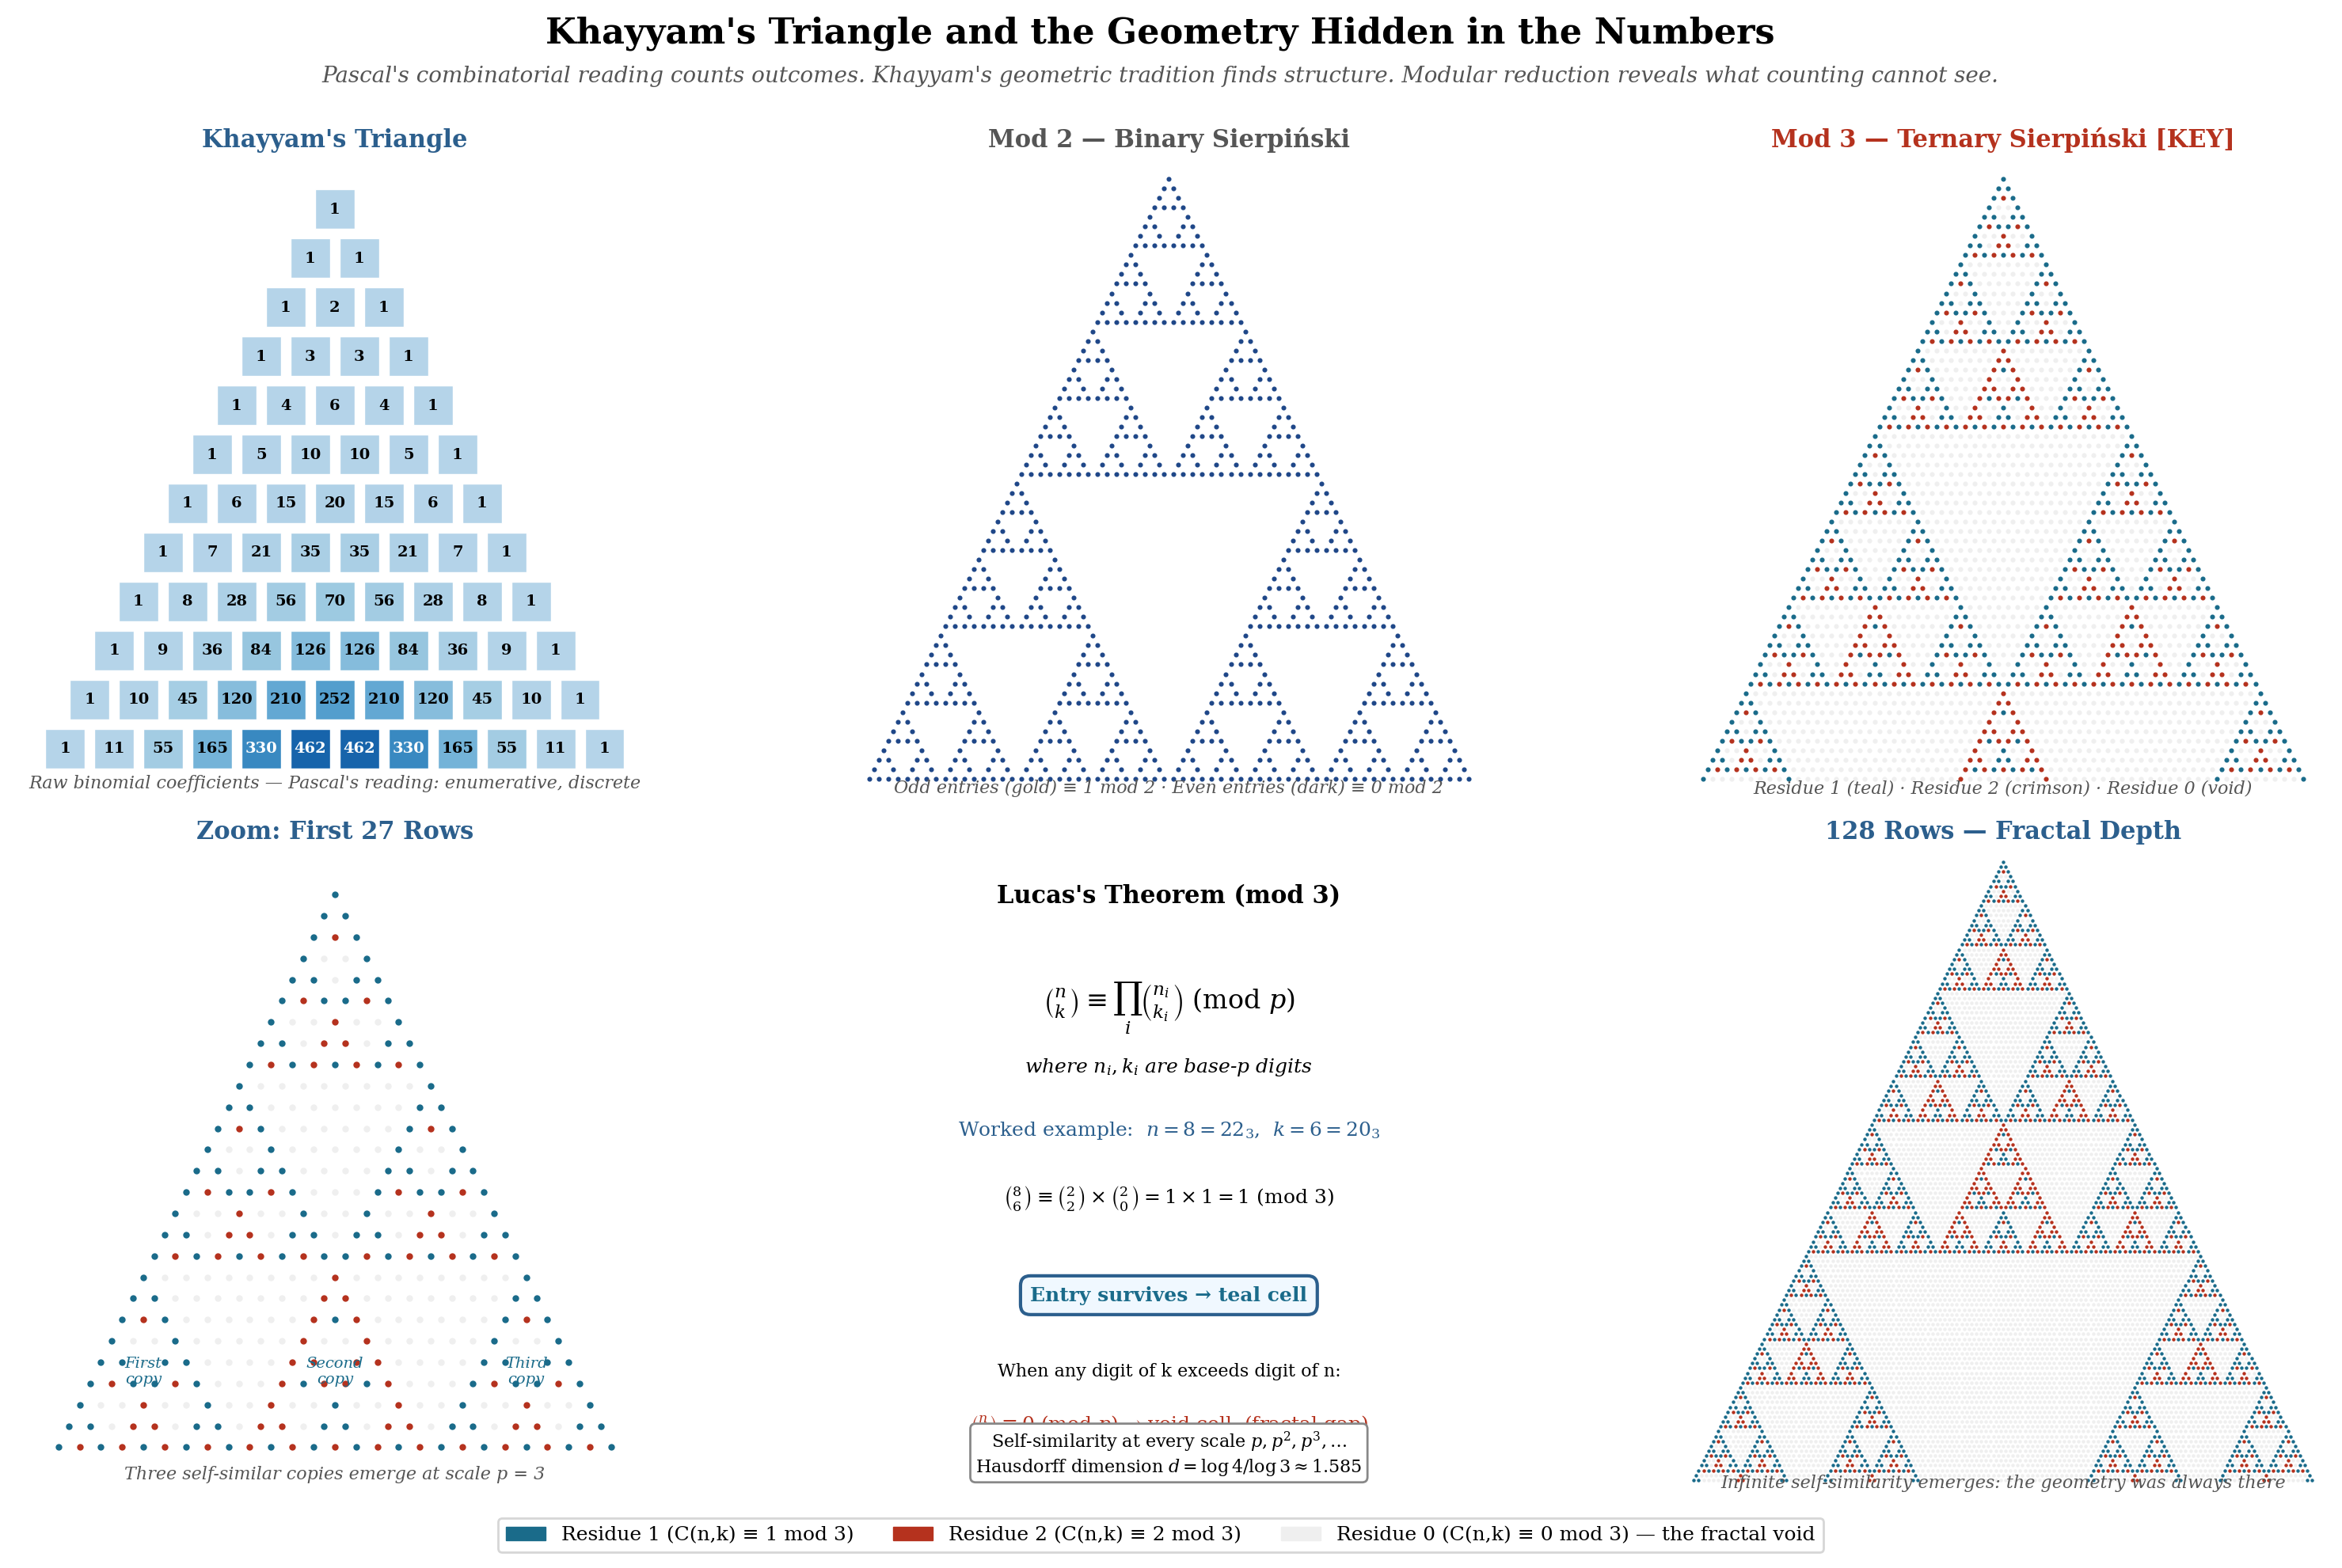
\includegraphics[width=\textwidth]{khayyam_sierpinski_academic.png}
\caption{From counting numbers to hidden geometry. \textit{Top row:} Khayyam's Triangle in raw form (12 rows), reduced modulo 2 (64 rows)---odd entries survive, even entries vanish, binary Sierpiński emerges (Hausdorff dimension $\log 3 / \log 2 \approx 1.585$), and reduced modulo 3 (64 rows)---residues 1 (teal) and 2 (crimson) survive, multiples of 3 collapse to void, ternary Sierpiński emerges (Hausdorff dimension $\log 4 / \log 3 \approx 1.262$). \textit{Bottom row:} First 27 rows showing three self-similar copies at scale $p=3$, Lucas's theorem mechanism explaining the fractal structure, and 128-row depth showing infinite self-similarity. Pascal's combinatorial question---\emph{how many outcomes?}---cannot see any of this. Khayyam's geometric question---\emph{what structure do these numbers encode?}---finds it immediately.}
\label{fig:fractal}
\end{figure}

\begin{thebibliography}{99}

\bibitem{khayyam1070}
O.~Khayyam, \emph{Maqālah fī al-jabr wa al-muqābalah}, Manuscript, Nishapur, Persia, c.~1070 CE.

\bibitem{altusi1265}
N.~D.~al-Tūsī, \emph{Sharḥ al-ishārāt}, Manuscript, Persia, 1265 CE.

\bibitem{yanghui1261}
Yang Hui, \emph{Xiangjie Jiuzhang Suanfa}, China, 1261 CE.

\bibitem{pascal1654}
B.~Pascal, \emph{Traité du triangle arithmétique}, G.~Desprez, Paris, 1654.

\bibitem{lucas1878}
É.~Lucas, Théorie des fonctions numériques simplement périodiques, \emph{Amer. J. Math.} \textbf{1} (1878), 184--196.

\bibitem{sierpinski1915}
W.~Sierpiński, Sur une courbe dont tout point est un point de ramification, \emph{C. R. Acad. Sci. Paris} \textbf{160} (1915), 302--305.

\bibitem{gardner1977}
M.~Gardner, Pascal's triangle, \emph{Sci. Amer.} \textbf{237}(6) (1977), 138--146.

\bibitem{wolfram1984}
S.~Wolfram, Geometry of binomial coefficients, \emph{Amer. Math. Monthly} \textbf{91} (1984), 566--570.

\bibitem{reiter1993}
C.~A.~Reiter, Determining the dimension of fractals generated by Pascal's triangle, \emph{Fibonacci Quart.} \textbf{31}(2) (1993), 112--120.

\bibitem{rashed2000}
R.~Rashed and B.~Vahabzadeh, \emph{Omar Khayyām the Mathematician}, Bibliotheca Persica Press, New York, 2000.

\bibitem{meeus2002}
J.~Meeus, The Gregorian Calendar and the Tropical Year, in \emph{More Mathematical Astronomy Morsels}, pp.~357--366, Willmann-Bell, Richmond, VA, 2002.

\bibitem{mathworld}
E.~W.~Weisstein, Pascal's Triangle, \emph{MathWorld---A Wolfram Web Resource}, \url{https://mathworld.wolfram.com/PascalsTriangle.html}.

\bibitem{ramanujan}
K.~Wakil, \emph{Ramanujan's dimensional forcing: a universal formula for sieve levels}, ARC Institute of Knowware, preprint, 2026.

\bibitem{eisenstein}
K.~Wakil, \emph{Ternary forcing on the hexagonal lattice: Eisenstein integers, cascade moduli, and level of distribution 5/8}, ARC Institute of Knowware, preprint, 2026.

\bibitem{w3condition}
K.~Wakil, \emph{Condition W3: absence of Siegel zeros for characters modulo $3^K$ via CM structure of $\mathbb{Z}[\omega]$}, ARC Institute of Knowware, preprint, 2026.

\bibitem{shannon}
K.~Wakil, \emph{The Shannon--Wakil effect: constitutional forcing as a universal pattern in information theory and prime arithmetic}, ARC Institute of Knowware, preprint, 2026.

\bibitem{spherical}
K.~Wakil, \emph{Spherical cow philosophy: a methodological framework for mathematical discovery}, ARC Institute of Knowware, preprint, 2026.

\end{thebibliography}

\end{document}
